\documentclass[parskip=full]{scrartcl}
\usepackage[utf8]{inputenc} % use utf8 file encoding for TeX sources
\usepackage[T1]{fontenc}    % avoid garbled Unicode text in pdf
\usepackage[german]{babel}  % german hyphenation, quotes, etc
\usepackage{hyperref}       % detailed hyperlink/pdf configuration
\hypersetup{                % ‘texdoc hyperref‘ for options
	pdftitle={Bericht},%
	bookmarks=true,%
}
\usepackage{graphicx}       % provides commands for including figures
\usepackage{csquotes}       % provides \enquote{} macro for "quotes"
\usepackage{scrpage2}
\usepackage{caption}
\usepackage{enumitem}
\pagestyle{scrheadings}
\usepackage{float}

%\clearscrheadfoot
\ohead{BPTI: Gruppe 03=\{Niklas Metz, Felix Bachmann\}, Bericht, WS 2017/18}
\title{BPTI: Bomberman in VHDL}

\begin{document}
	\maketitle
	\section{Beschreibung der Entities}
		\subsection{Bomberman}
		
		\subsection{Game\_mechanic}
		
		\subsection{Game\_state}
		
		\subsection{player\_ent}
			%TODO blockdiagramm
			\subsubsection{movement\_ent}
			
			\subsubsection{clk\_movement\_ent}
				Die Entity clk\_movement\_ent ist ein Clock Divider, die Architecture wird funktional beschrieben. Die Entity wird genutzt, um die Geschwindigkeit der Bewegung der Spieler zu steuern. Es wird alle 78125 Originaltakte die Ausgabe Ausgabe negiert. Da in unserem Design die VGA-Clock genutzt wird, wird somit alle $\frac{78125 * 2}{25.175 * 10^6}s \approx 6.2ms$ ein Takt erzeugt. Dies hat zur Folge, dass bei ständiger Bewegung eines Spielers in die gleiche Richtung, die pro steigender Takt-Flanke des ausgegebenen Takts stattfindet, die Bewegung vom linken bis zum rechten Rand des Spielfelds (480 Pixel) $480 * 6.2 ms \approx 2.98 s$ dauert. Diesen Wert haben wir bei BombermanGB über einen Emulator gemessen und \enquote{rückwärts} den nötigen Zähler, also 78125, bestimmt.
			\subsubsection{bomb\_ent}
				%TODO simulations-screenshot
		\subsection{Pixel\_gen}
		
		\subsection{RGB\_assign}
		
		\subsection{Sprites}
			In den beiden Entities PlayerROM und SpriteROM befinden sich Sprites, die in Abhängigkeit des aktuellen Zustands der Arena, der Spieler und der Bomben RGB-Werte an den VGA-Controller ausgeben. Dazu befinden sich in den beiden Entities PlayerROM und SpriteROM pro Sprite (es existieren Sprites für: Spieler 1, Spieler 2, leerer Block, zerstörbarer Block, unzerstörbarer Block, Bombe, Explosion) ein zweidimensionales konstantes Array (wird synthetisiert als ROM). Diese Arrays sind jeweils 32 * 384 Bit groß. \newline
			Die Größe ergibt sich folgendermaßen: Die Kacheln des Spielfeldes sowie die Quellsprites haben eine Größe von 32 * 32 Pixel. Da für jeden Farbkanal des VGA-Ausgangs 4 Bit zur Verfügung stehen haben wir in dem Array den RGB-Wert jedes Pixels mit 3 * 4 Bit (also 3 Hex-Werte) kodiert. So kommen 32 Zeilen mit jeweils 
			3 * 4 * 32 = 384 Bit zustande. \newline
			Die Sprites haben wir aus einem Sprite-Sheet von opengameart (\url{https://opengameart.org/sites/default/files/DungeonCrawl_ProjectUtumnoTileset.png}) ausgeschnitten und mithilfe eines Java-Programmes, welches im Abgabe-Verzeichnis zu finden ist und im folgenden kurz beschrieben wird, in VHDL-Arrays umgewandelt.
			\subsubsection{SpriteExtractor.java}
				Das Java-Programm bekommt als Kommandozeilenargumente die Pfade zu den 32 * 32 Pixel großen Sprites. Über jedes der Sprites wird pixelweise iteriert und für jeden Pixel der RGB-Wert ausgelesen. Daraus werden die Werte der einzelnen Farbkanäle bestimmt, welche anschließend normiert werden, da auf dem FPGA nur 4 Bit pro Farbkanal nutzbar sind. Die normierten Werte werden in Hex-Character umgewandelt und auf der Konsole ausgegeben, sodass die RGB-Kanäle jedes Pixels mit 3 Hex-Charactern  dargestellt werden. Die Ausgabe erfolgt in der Form von 32 komma-separierten std\_logic\_vectoren der Länge 384.
			\subsubsection{SpriteROM}
				Die Entity SpriteROM wird mit einer Architecture funktional beschrieben. Abhängig von der sprite\_id wird mittels sprite\_row und sprite\_col asynchron auf die verschiedenen Arrays zugegriffen. Die sprite\_id orientiert sich hierbei an den Kodierungen des Spielfeldes (siehe game\_state, z.B. leerer Block = x0). Ist keine gültige id gesetzt (also id > x1 und id < xD), wird RGB schwarz ausgegeben.
			\subsubsection{PlayerROM}
				Die Entity PlayerROM ist hinter SpriteROM geschaltet und überscheibt die RGB-Werte, die von SpriteROM ausgegeben werden, wenn sich im aktuellen Pixel des Bildes ein Spieler befindet. In PlayerROM befinden sich zwei konstante Arrays, die in der gleichen Form wie in SpriteROM die Sprites für die Spieler enthalten. PlayerROM bekommt zum Auslesen der Arrays eine id (x2 für Spieler 1, x3 für Spieler 2), sowie die x- und y-Position des Spielers im aktuell betrachteten Pixels. Ist die id gültig, wird der RGB-Wert des entsprechenden Sprites gelesen und ausgegeben. Überlappen sich beide Spieler, so wird stets Spieler 1 gezeichnet.
				Ist keine gültige id gesetzt (also id > x3 oder id < x2), wird der RGB-Wert von SpriteROM durchgeschaltet.
				Hat ein Pixel den (in unseren Sprites speziellen) RGB-Wert xEEE wird ebenfalls der RGB-Wert von SpriteROM durchgeschaltet. Dies sorgt dafür, dass die Spielfiguren erkennbare Strukturen haben (Spieler sind keine Kacheln) und sich sichtbar vor einem Hintergrund bewegen.
		
		\subsection{sync\_gen\_ent}
			Die Entity sync\_gen\_ent wird mit einer Architecture strukturell beschrieben durch die Unterkomponenten hsync und vsync. In dieser Entity werden die Signale für den VGA-Controller generiert (also hsync und vsync). Desweiteren werden zum Setzen der Pixel die aktuelle row und column ausgegeben.
			An dieser Stelle sei auf das VGA-Übungsblatt und den Bericht darüber verwiesen. Wir haben unsere Lösung von dem Übungsblatt für das Projekt übernommen und im Laufe des Projekts nichts an der Entity inklusive Unterkomponenten gerändert.
			\begin{figure}[H]
				\centering
				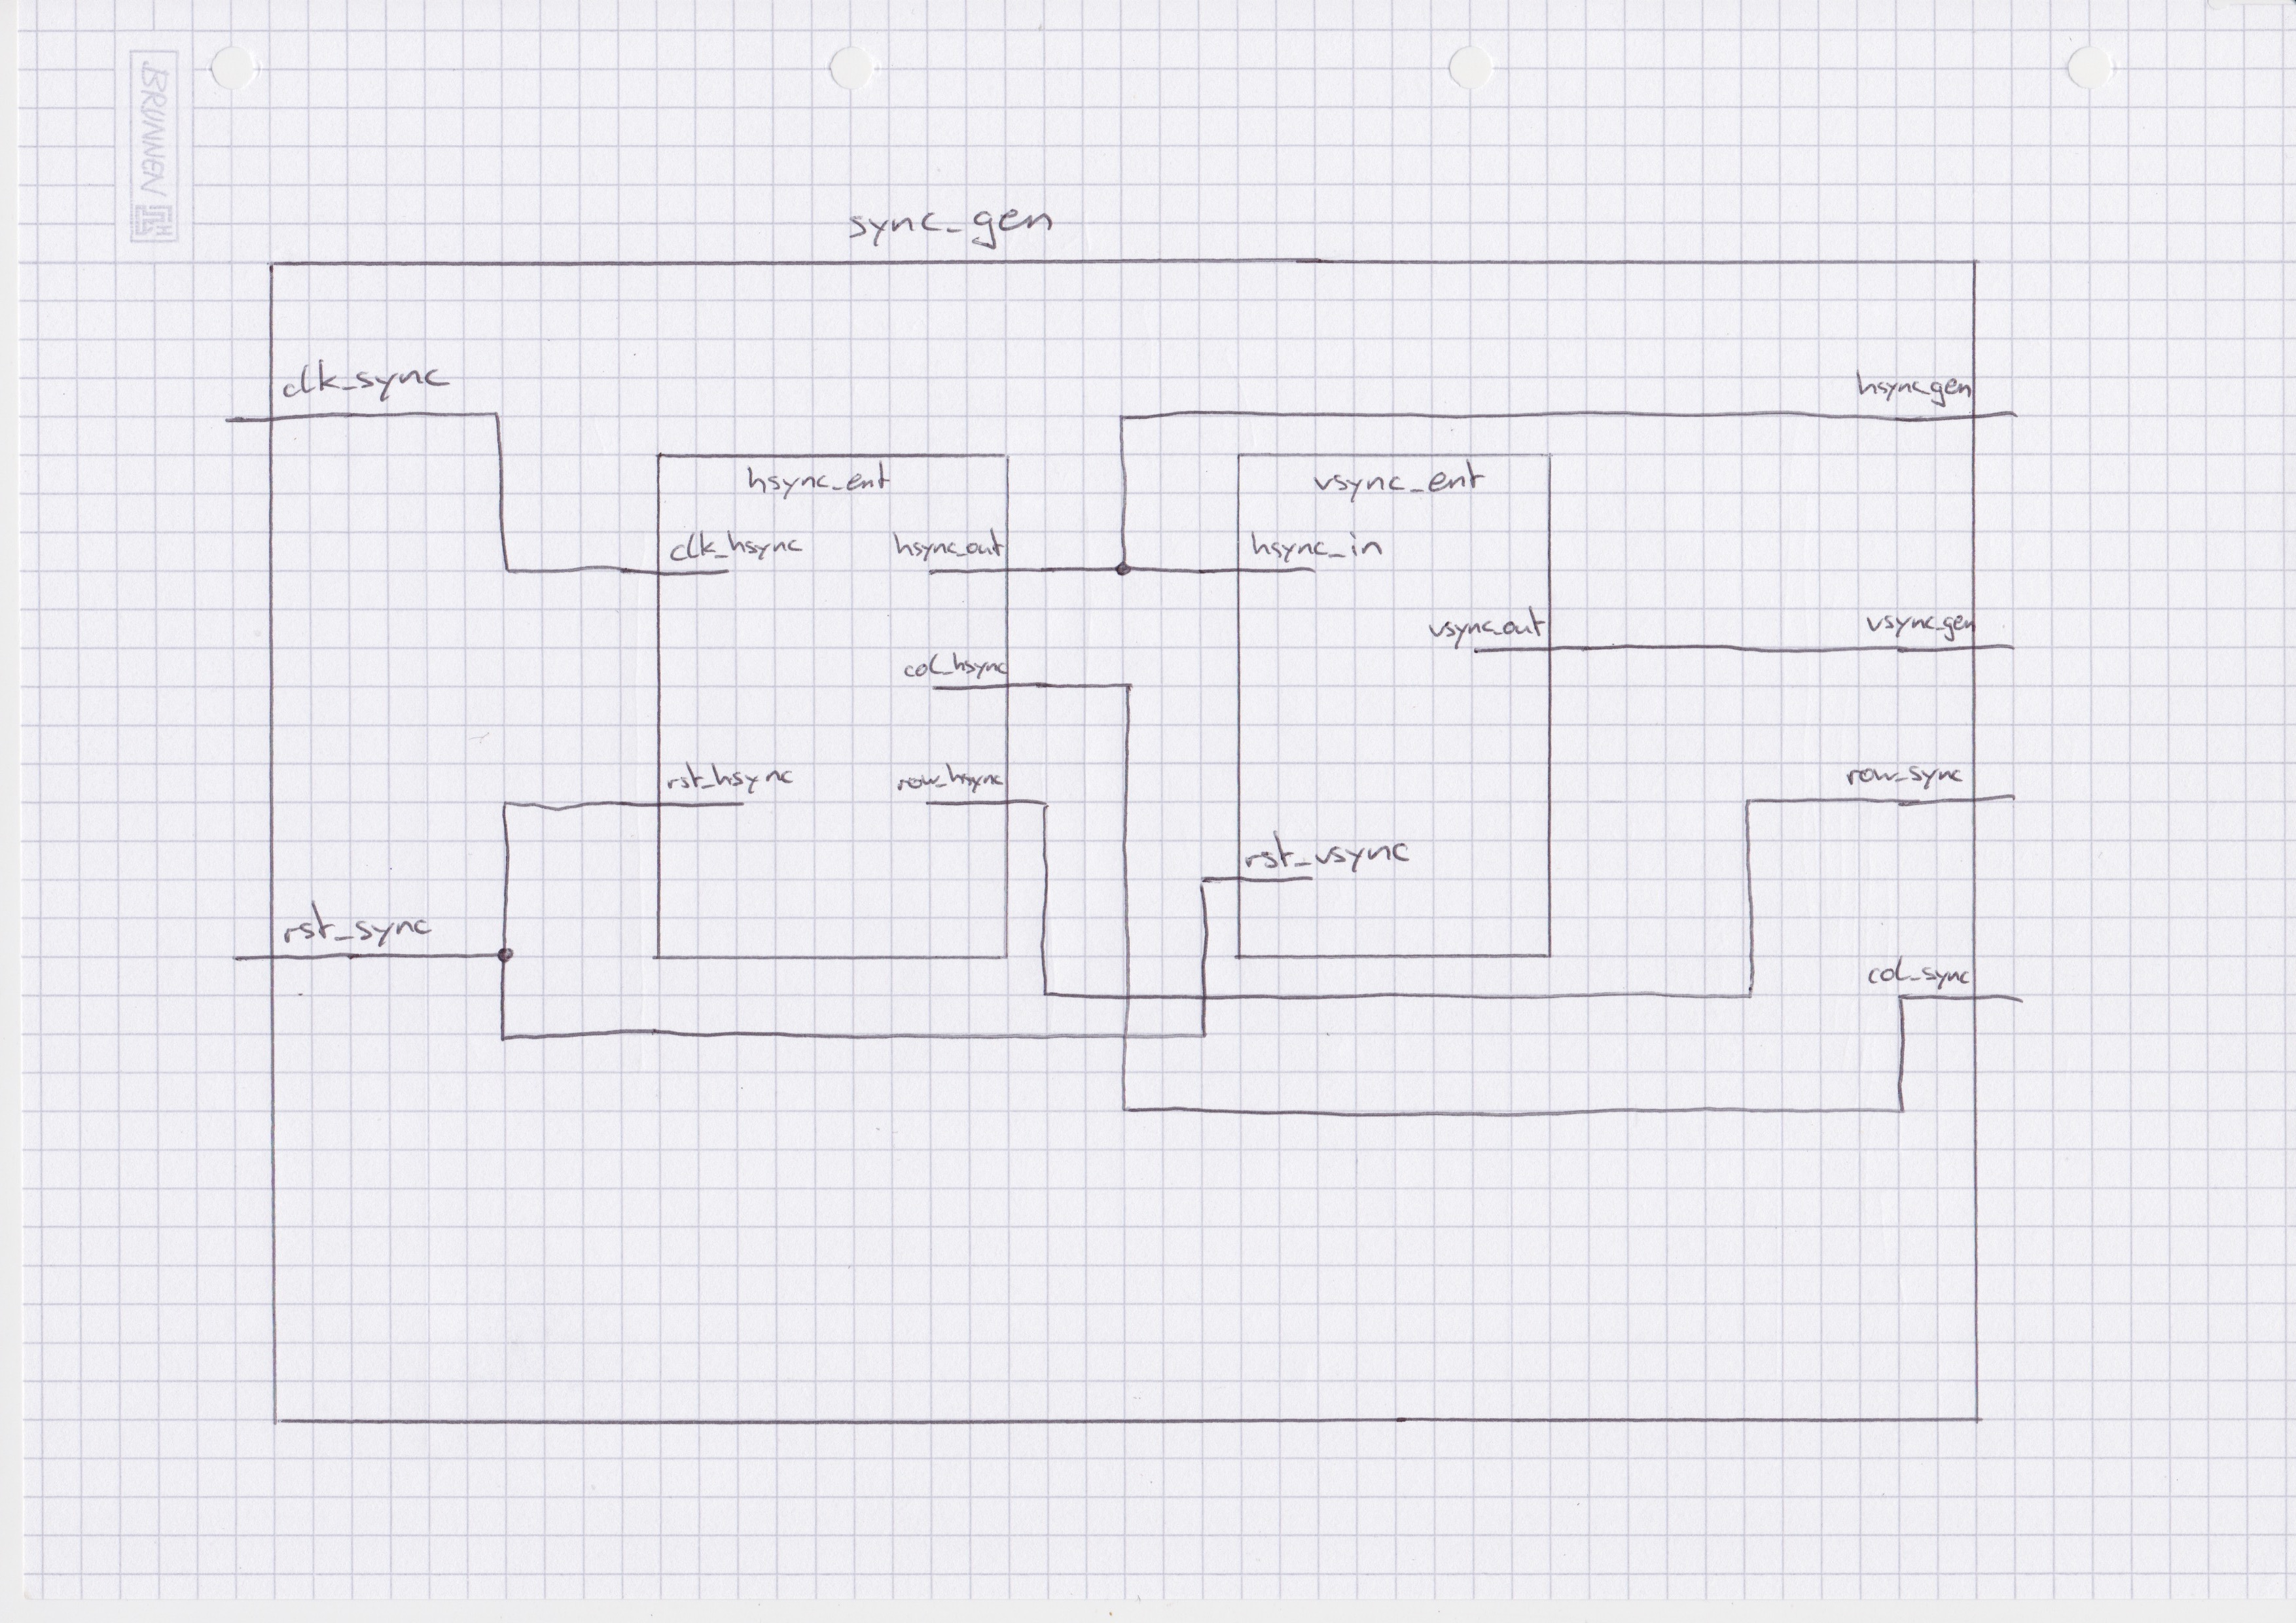
\includegraphics[scale=0.1]{./bilder/Sync_gen.jpeg}
			\end{figure}
		
	\section{Probleme}
		\subsection{Bomberman}
		
		\subsection{Game\_mechanic}
		
		\subsection{Game\_state}
		
		\subsection{Player}
		
		\subsection{Movement}
		
		\subsection{Mov\_clk}
		
		\subsection{Bomb}
		
		\subsection{Pixel\_gen}
		
		\subsection{RGB\_assign}
		
		\subsection{Sprites}
			%TODO farben gefixt bekommen?
		
		\subsection{sync\_gen\_ent}
			Ein Problem, das schon bei der Lösung des Übungsblatts aufgetaucht ist, hat sich auch durch das Projekt gezogen.
			Die VGA-Ausgabe funktioniert nicht an allen Monitoren ordnungsgemäß (flackern). An unserem Test-Monitor hat die VGA-Ausgabe nach einigen Einstellungen jedoch funktioniert.
\end{document}